\usepackage{pgf}
\usepackage{tikz}
\usetikzlibrary{arrows,automata,fit}

\newcommand{\ejemplografo}{
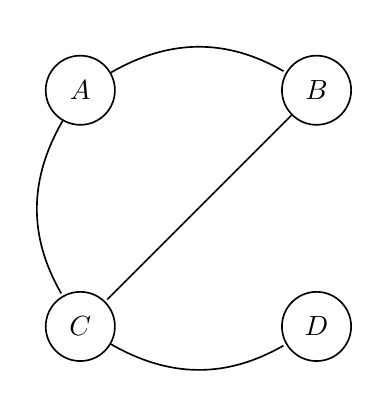
\begin{tikzpicture}[>=stealth',shorten >=1pt,auto,node distance=3cm,semithick]
  \tikzstyle{every state}=[draw=black,text=black]

  \node[state]         (A)                    {$A$};
  \node[state]         (B) [right of=A]       {$B$};
  \node[state]         (C) [below of=A]       {$C$};
  \node[state]         (D) [right of=C]       {$D$};
  
  \path (A) edge  [bend left]   node {}  (B)
            edge  [bend right]  node {}  (C)
        (B) edge                node {}  (C)
        (C) edge  [bend right]  node {}  (D);
\end{tikzpicture}}